\renewcommand{\appendixname}{Anexo}
\renewcommand{\thechapter}{\Alph{chapter}}

% Comando para iniciar la sección de anexos en el índice
\newcommand{\initappendix}{%
  \addcontentsline{toc}{chapter}{Anexo}%
}

% Comando para cada anexo individual
\newcommand{\anexo}[1]{%
  \refstepcounter{chapter}%
  \chapter*{Anexo \thechapter: #1}%
  \addcontentsline{toc}{section}{Anexo \thechapter: #1}%
  \markboth{Anexo \thechapter: #1}{}%
}

\initappendix

\ifdeliveryannexschedule
	\anexo{Cronograma de Actividades}\label{anexo:cronograma}

El desarrollo del proyecto avanza conforme a lo planificado para el hito de entrega del 25\%. Las actividades de definici\'on, marco te\'orico y estado del arte fueron completadas entre abril y mayo de 2026, sin desv\'{\i}os significativos respecto del calendario inicial. La investigaci\'on con usuarios (encuestas y entrevistas) se mantiene planificada para junio y julio de 2026, en l\'{\i}nea con el alcance acordado para la entrega del 50\%, de modo que el presente informe pueda concentrarse en los antecedentes conceptuales y la fundamentaci\'on de la brecha de investigaci\'on.

\begin{landscape}
\begin{figure}[ht]
	\centering
	\footnotesize
	\begin{ganttchart}[
		x unit=1.05cm,
		y unit chart=0.55cm,
		time slot format=isodate,
		time slot unit=month,
		title/.style={draw=none, fill=gray!25},
		title label font=\small\bfseries,
		bar label font=\scriptsize,
		group label font=\small\bfseries,
		bar/.style={fill=blue!35, draw=blue!60},
		bar complete/.style={fill=green!45, draw=green!60!black},
		bar height=0.55,
		group height=0.35,
		group peaks height=0.2,
		milestone height=0.45,
		progress label text={},
		canvas/.style={draw=none},
		vgrid={*1{draw=gray!20}},
		hgrid={*1{draw=gray!20}}
	]{2026-04-01}{2026-11-30}
		\gantttitlecalendar{year, month=shortname} \\
		\ganttgroup{Antecedentes (hito 25\%)}{2026-04-01}{2026-05-31} \\
		\ganttbar[progress=100]{Propuesta y definición}{2026-04-01}{2026-04-30} \\
		\ganttbar[progress=100]{Marco teórico}{2026-04-15}{2026-05-15} \\
		\ganttbar[progress=100]{Estado del arte}{2026-05-01}{2026-05-31} \\
		\ganttmilestone{Entrega 25\%}{2026-05-31} \\
		\ganttgroup{Desarrollo (hito 50\%)}{2026-06-01}{2026-07-31} \\
		\ganttbar{Investigación con usuarios}{2026-06-01}{2026-06-30} \\
		\ganttbar{Ingeniería de datos}{2026-06-01}{2026-07-15} \\
		\ganttbar{Modelado XGBoost}{2026-07-01}{2026-07-31} \\
		\ganttmilestone{Entrega 50\%}{2026-07-31} \\
		\ganttgroup{Integración (hito 75\%)}{2026-08-01}{2026-09-30} \\
		\ganttbar{Explicabilidad SHAP}{2026-08-01}{2026-08-31} \\
		\ganttbar{Backend API (.NET)}{2026-08-01}{2026-09-15} \\
		\ganttbar{Frontend (React)}{2026-08-15}{2026-09-30} \\
		\ganttbar{Despliegue en AWS}{2026-09-01}{2026-09-30} \\
		\ganttmilestone{Entrega 75\%}{2026-09-30} \\
		\ganttgroup{Cierre (hito 100\%)}{2026-10-01}{2026-11-30} \\
		\ganttbar{Validación y métricas}{2026-10-01}{2026-10-31} \\
		\ganttbar{Documentación final}{2026-11-01}{2026-11-30} \\
		\ganttmilestone{Entrega final}{2026-11-30}
	\end{ganttchart}
	\caption{Cronograma de actividades del proyecto y estado de avance al hito del 25\%.}
	\label{fig:cronograma}
\end{figure}
\end{landscape}

\fi
\ifdeliveryannexsurveys
	\anexo{Resultados de la encuesta}\label{anexo:encuesta}

\enc{Entre junio y octubre de 2026 se recolectaron 248 respuestas v\'alidas de un formulario en l\'{\i}nea sobre prevenci\'on y seguridad laboral, aplicado a trabajadores de distintos sectores y tama\~nos de establecimiento en Argentina.}
Este anexo presenta la ficha t\'ecnica y los gr\'aficos por pregunta.
La interpretaci\'on de los resultados est\'a en la secci\'on Investigaci\'on con usuarios del Cap\'itulo~\ref{ch:descripcion}.

\subsection*{Ficha t\'ecnica}

\begin{description}[style=nextline, leftmargin=3.4cm, labelwidth=3.0cm]
	\item[Instrumento] Formulario en l\'{\i}nea de Google Forms sobre prevenci\'on y seguridad laboral.
	\item[Per\'{\i}odo] \enc{Junio a octubre de 2026.}
	\item[Muestra] \enc{248 respuestas v\'alidas.}
	\item[Poblaci\'on] Trabajadores de distintos sectores y tama\~nos de establecimiento en Argentina.
\end{description}

\subsection*{P1: Sector laboral}

\begin{figure}[htbp]
	\centering
	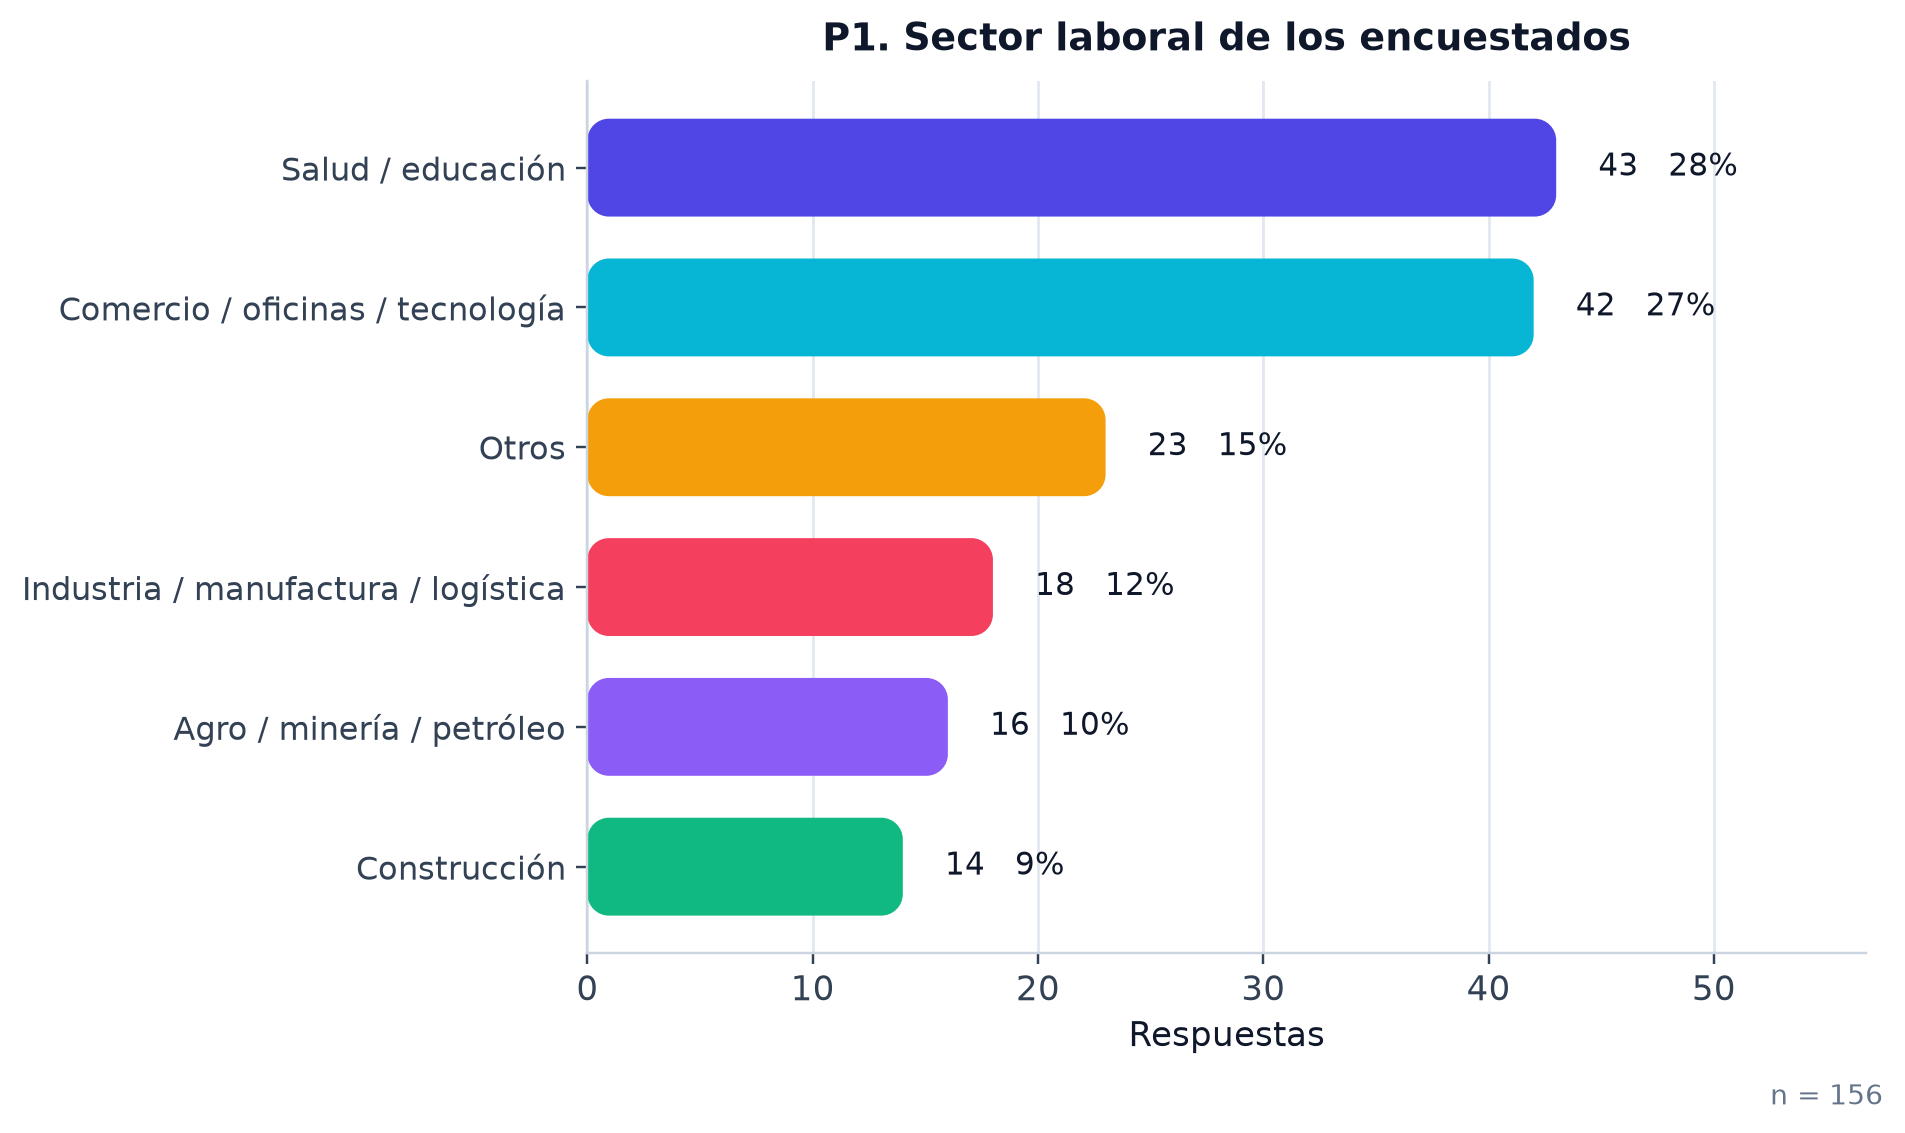
\includegraphics[width=0.92\textwidth]{figures/encuesta/p1_sector.png}
	\caption{\enc{Distribuci\'on por sector. Las categor\'{\i}as libres de baja frecuencia se agruparon en Otros. $n=248$.}}
	\label{fig:enc-p1}
\end{figure}

\enc{Comercio, oficinas y tecnolog\'{\i}a, 31\,\%. Salud y educaci\'on, 25\,\%. Otros, 19\,\%. Industria y log\'{\i}stica, 10\,\%. Agro, miner\'{\i}a y petr\'oleo, 9\,\%. Construcci\'on, 8\,\%.}

\subsection*{P2: Tama\~no del establecimiento}

\begin{figure}[htbp]
	\centering
	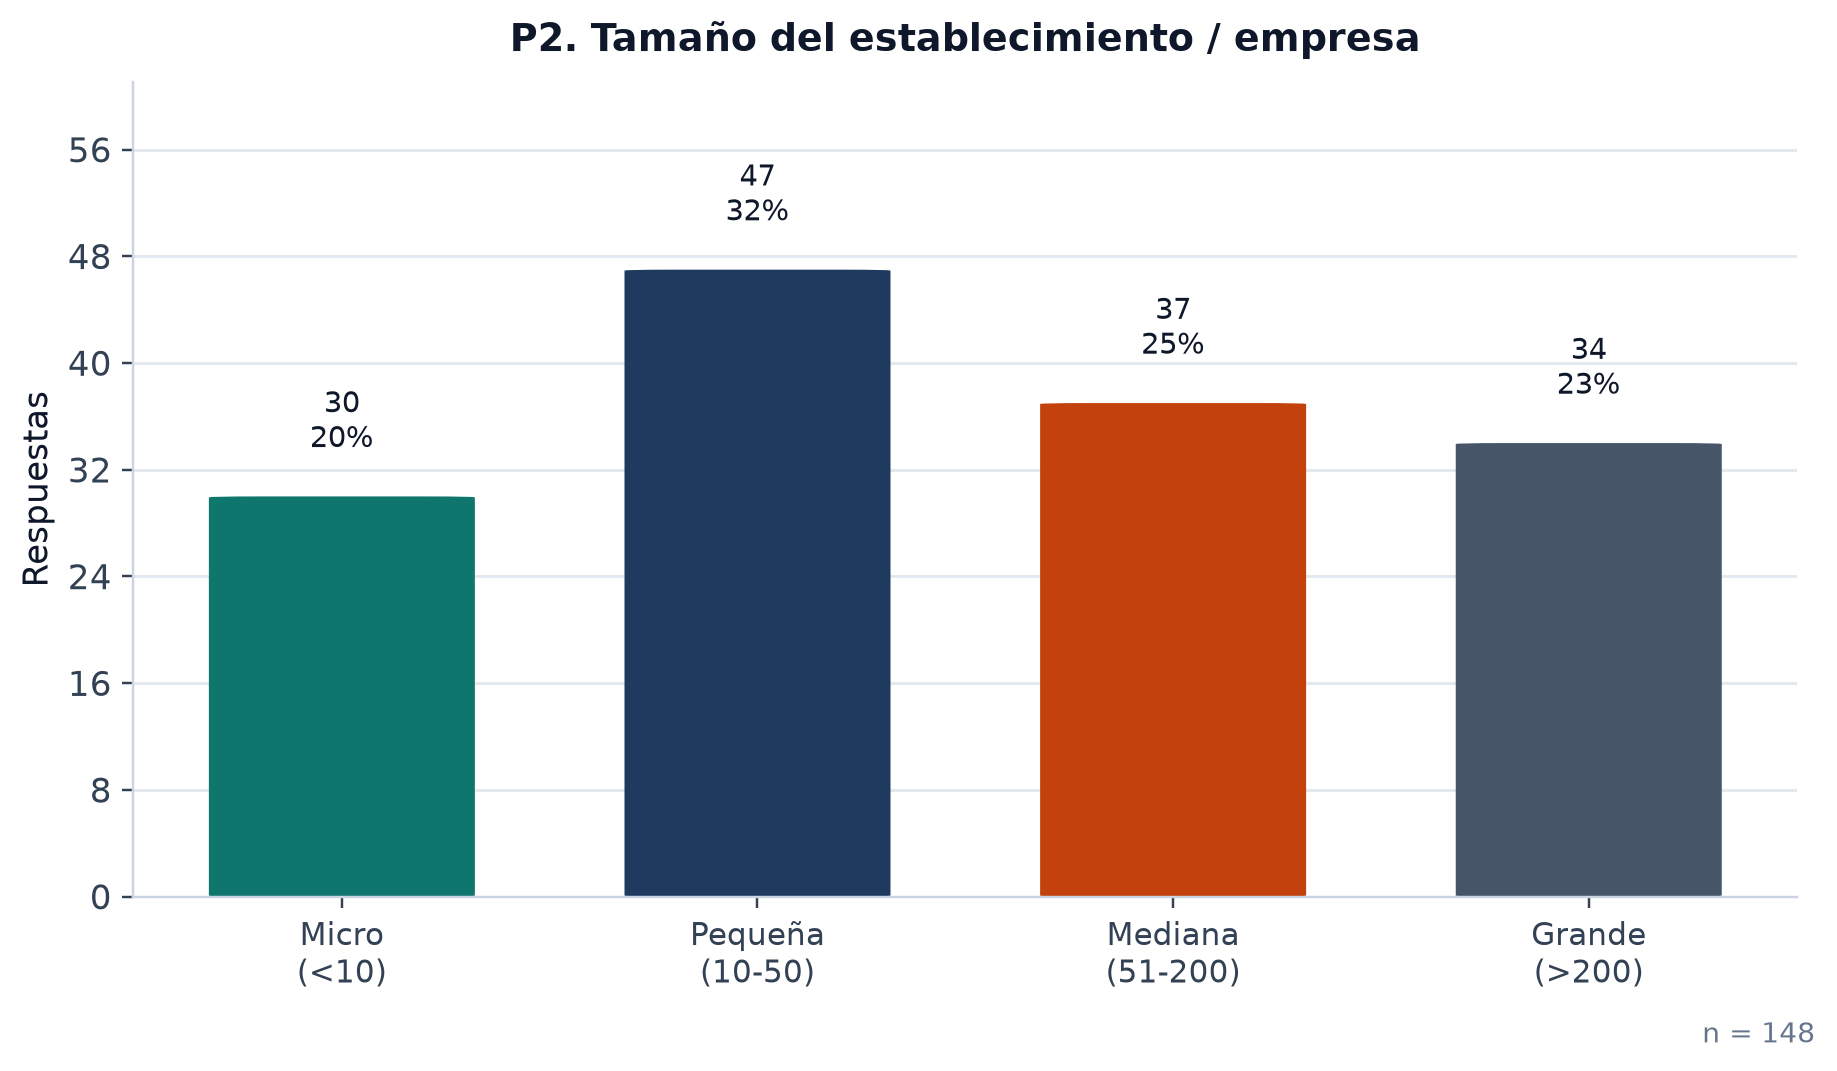
\includegraphics[width=0.92\textwidth]{figures/encuesta/p2_tamanio.png}
	\caption{\enc{Tama\~no aproximado de la empresa o establecimiento. $n=232$.}}
	\label{fig:enc-p2}
\end{figure}

\enc{Micro, 23\,\%. Peque\~na, 29\,\%. Mediana, 25\,\%. Gran empresa, 23\,\%.
Diecis\'eis respuestas de P1 no informaron tama\~no.}

\subsection*{P3: Conocimiento de la ART y auditor\'{\i}as}

\begin{figure}[htbp]
	\centering
	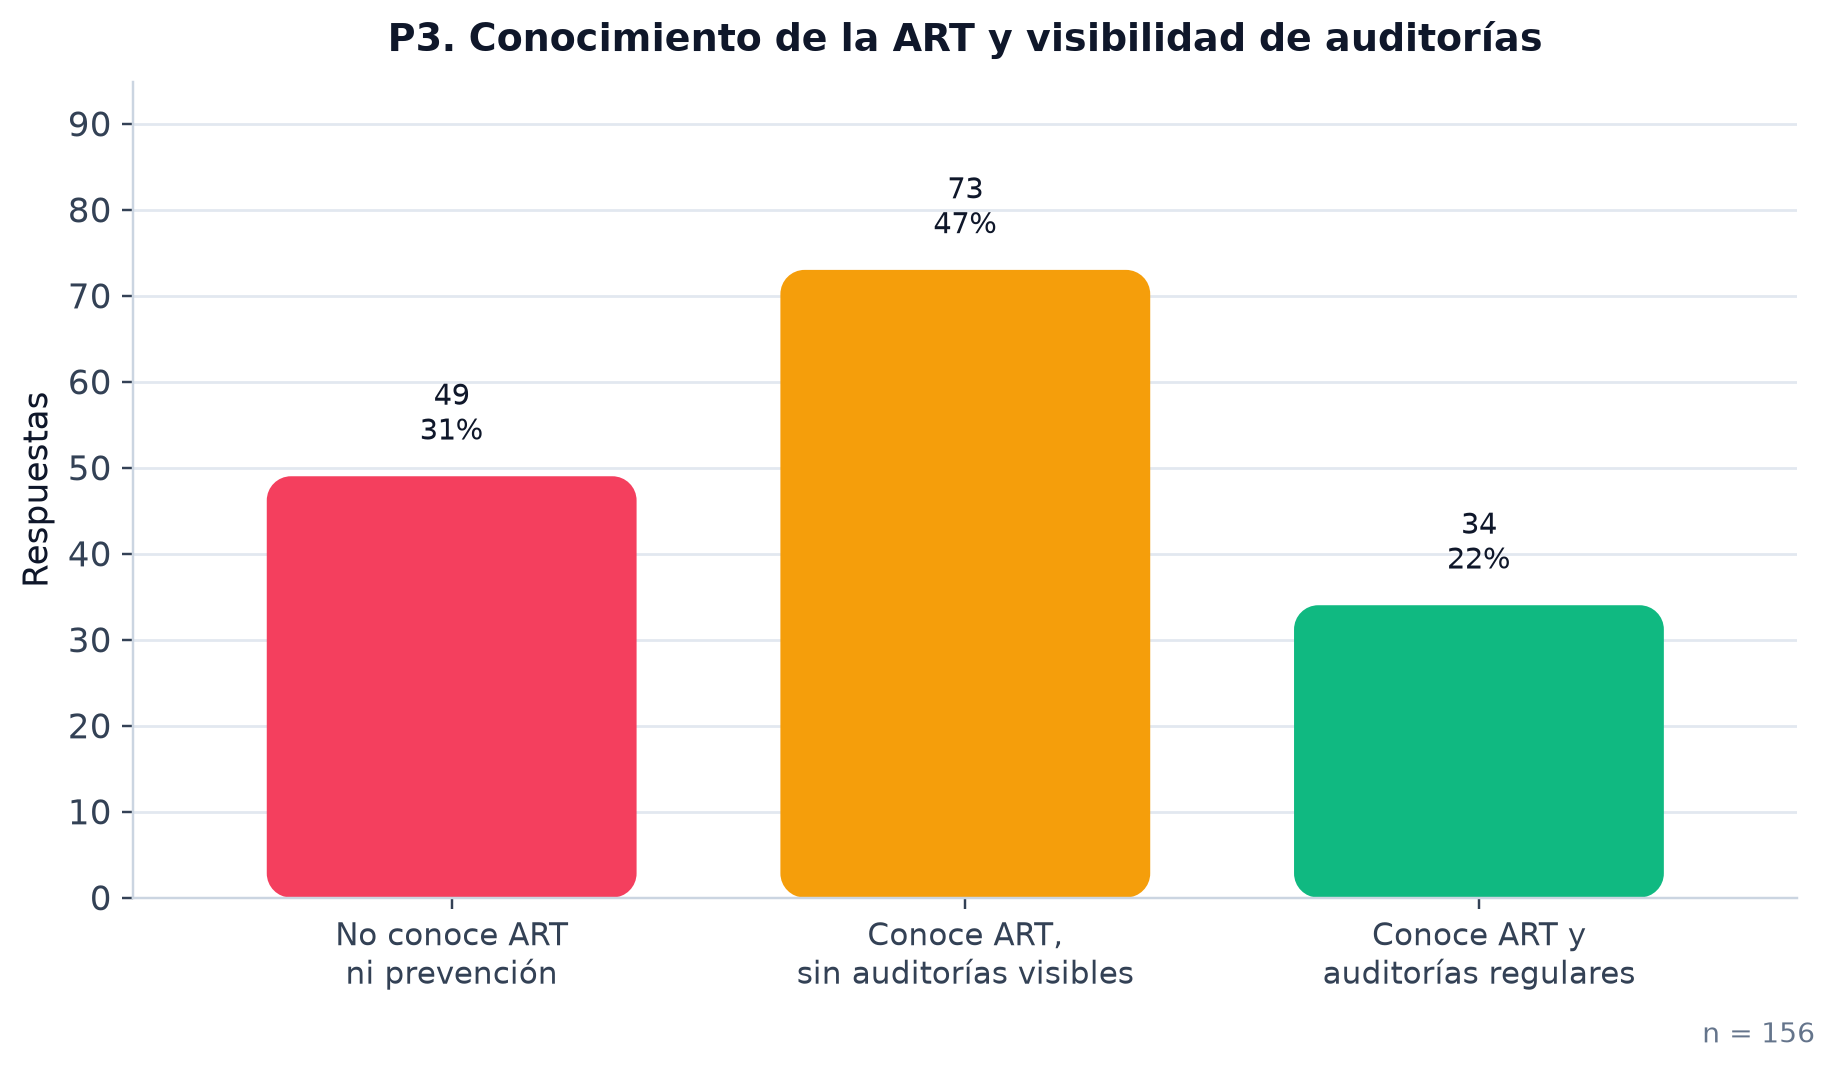
\includegraphics[width=0.92\textwidth]{figures/encuesta/p3_art.png}
	\caption{\enc{Conocimiento de la ART y visibilidad de auditor\'{\i}as preventivas. $n=248$.}}
	\label{fig:enc-p3}
\end{figure}

\enc{El 35\,\% no tiene idea de qu\'e ART lo cubre ni si hay prevenci\'on.
El 44\,\% conoce la ART pero nunca vio auditor\'{\i}as o inspecciones.
El 21\,\% conoce la ART y reporta auditor\'{\i}as regulares.}

\subsection*{P4: Capacitaciones y medidas de seguridad}

\begin{figure}[htbp]
	\centering
	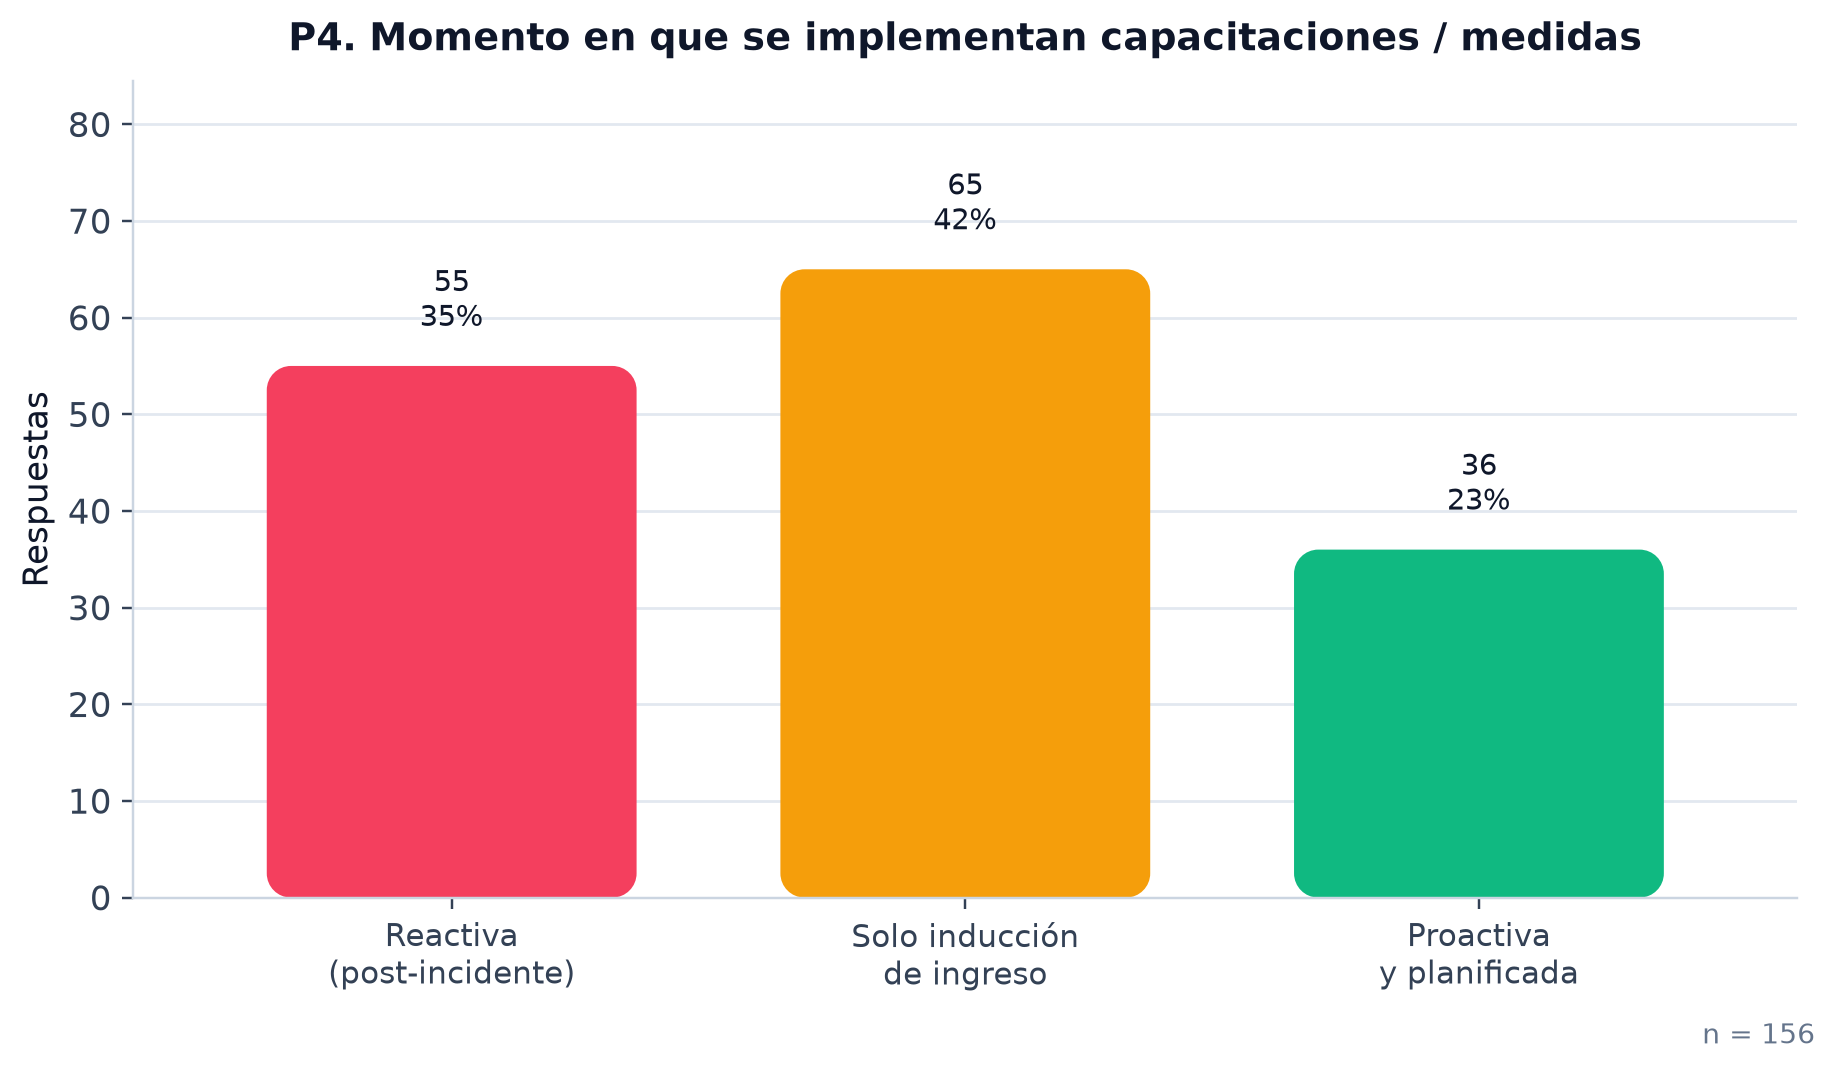
\includegraphics[width=0.92\textwidth]{figures/encuesta/p4_capacitaciones.png}
	\caption{\enc{Momento predominante de implementaci\'on de capacitaciones o medidas. $n=248$.}}
	\label{fig:enc-p4}
\end{figure}

\enc{El 38\,\% las sit\'ua despu\'es de un incidente.
El 40\,\% las limita a la inducci\'on de ingreso.
El 23\,\% describe un enfoque proactivo y planificado a lo largo del a\~no.}

\subsection*{P5: Preparaci\'on percibida, escala 1 a 5}

\begin{figure}[htbp]
	\centering
	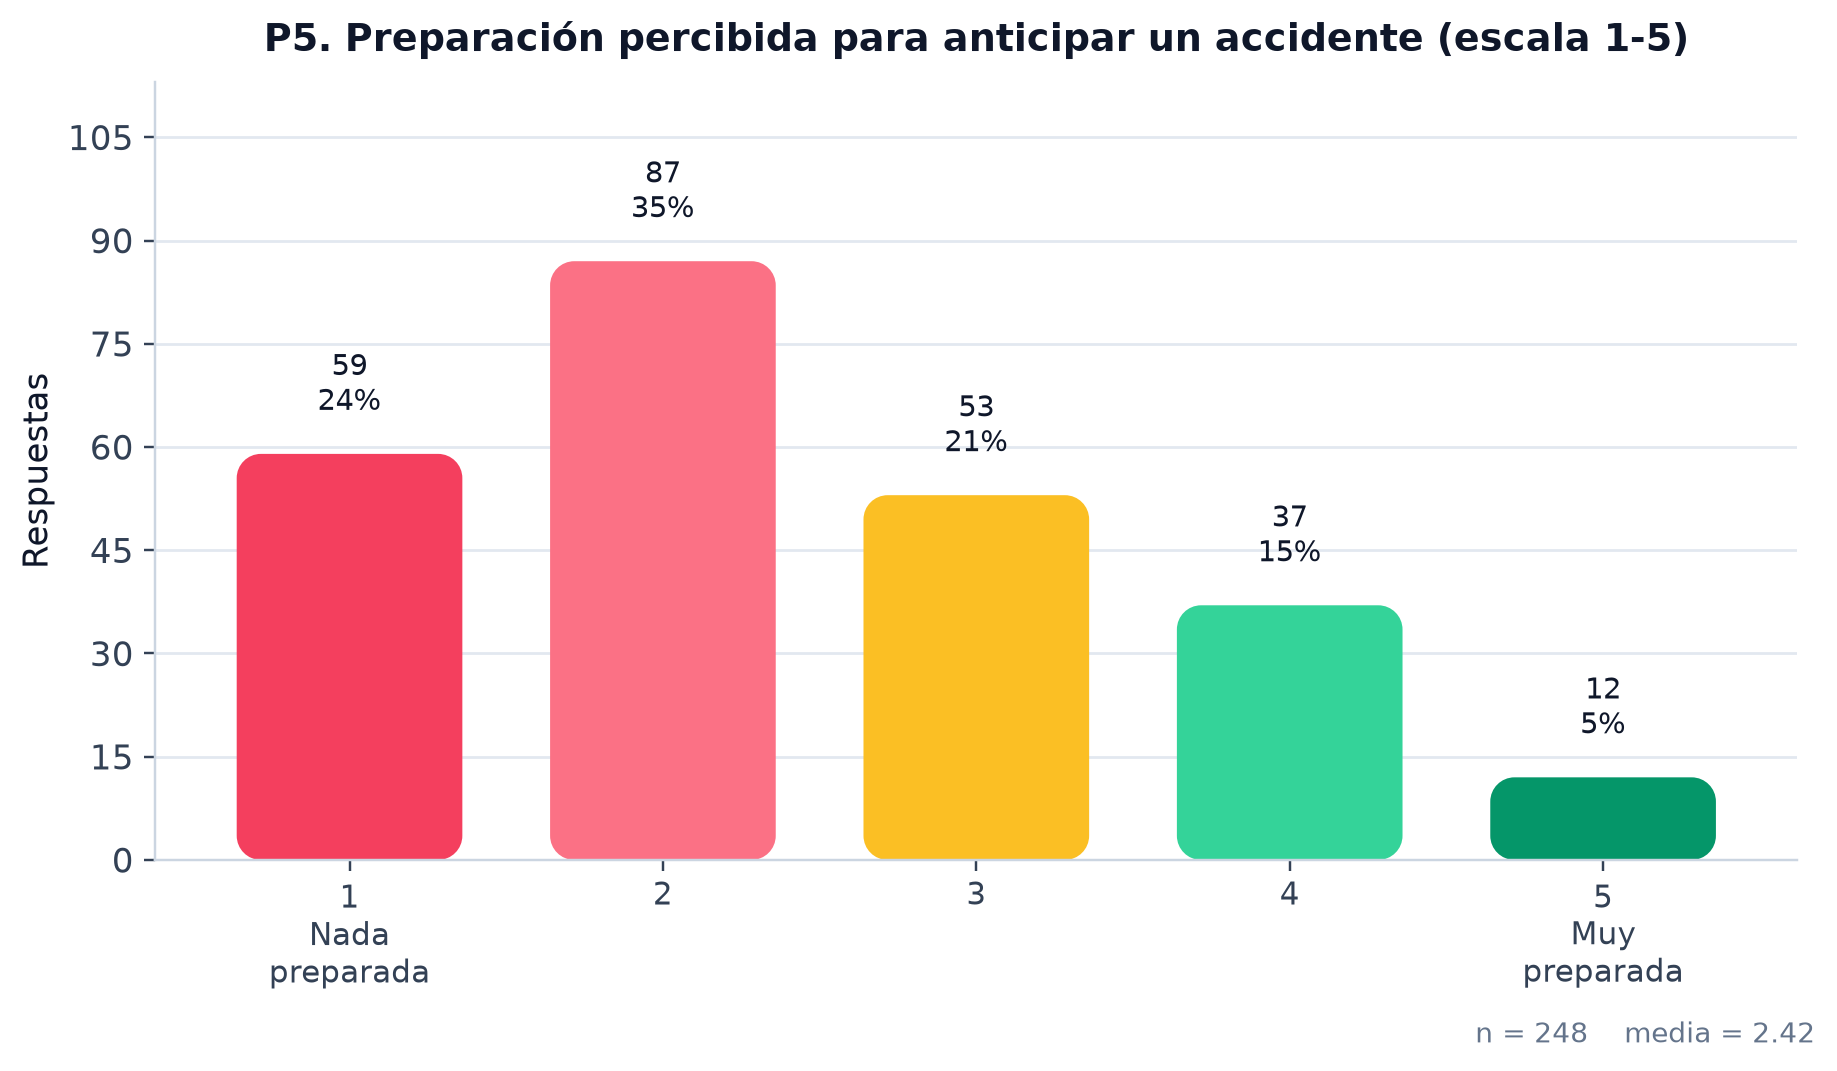
\includegraphics[width=0.92\textwidth]{figures/encuesta/p5_preparacion.png}
	\caption{\enc{Autoevaluaci\'on de preparaci\'on de la empresa para anticipar un accidente. $n=248$; media 2,42.}}
	\label{fig:enc-p5}
\end{figure}

\enc{Media 2,42. Mediana 2.
El 59\,\% elige 1 o 2.
El 5\,\% elige el m\'aximo, 5.}

\subsection*{P6: Experiencia de accidente o enfermedad profesional}

\begin{figure}[htbp]
	\centering
	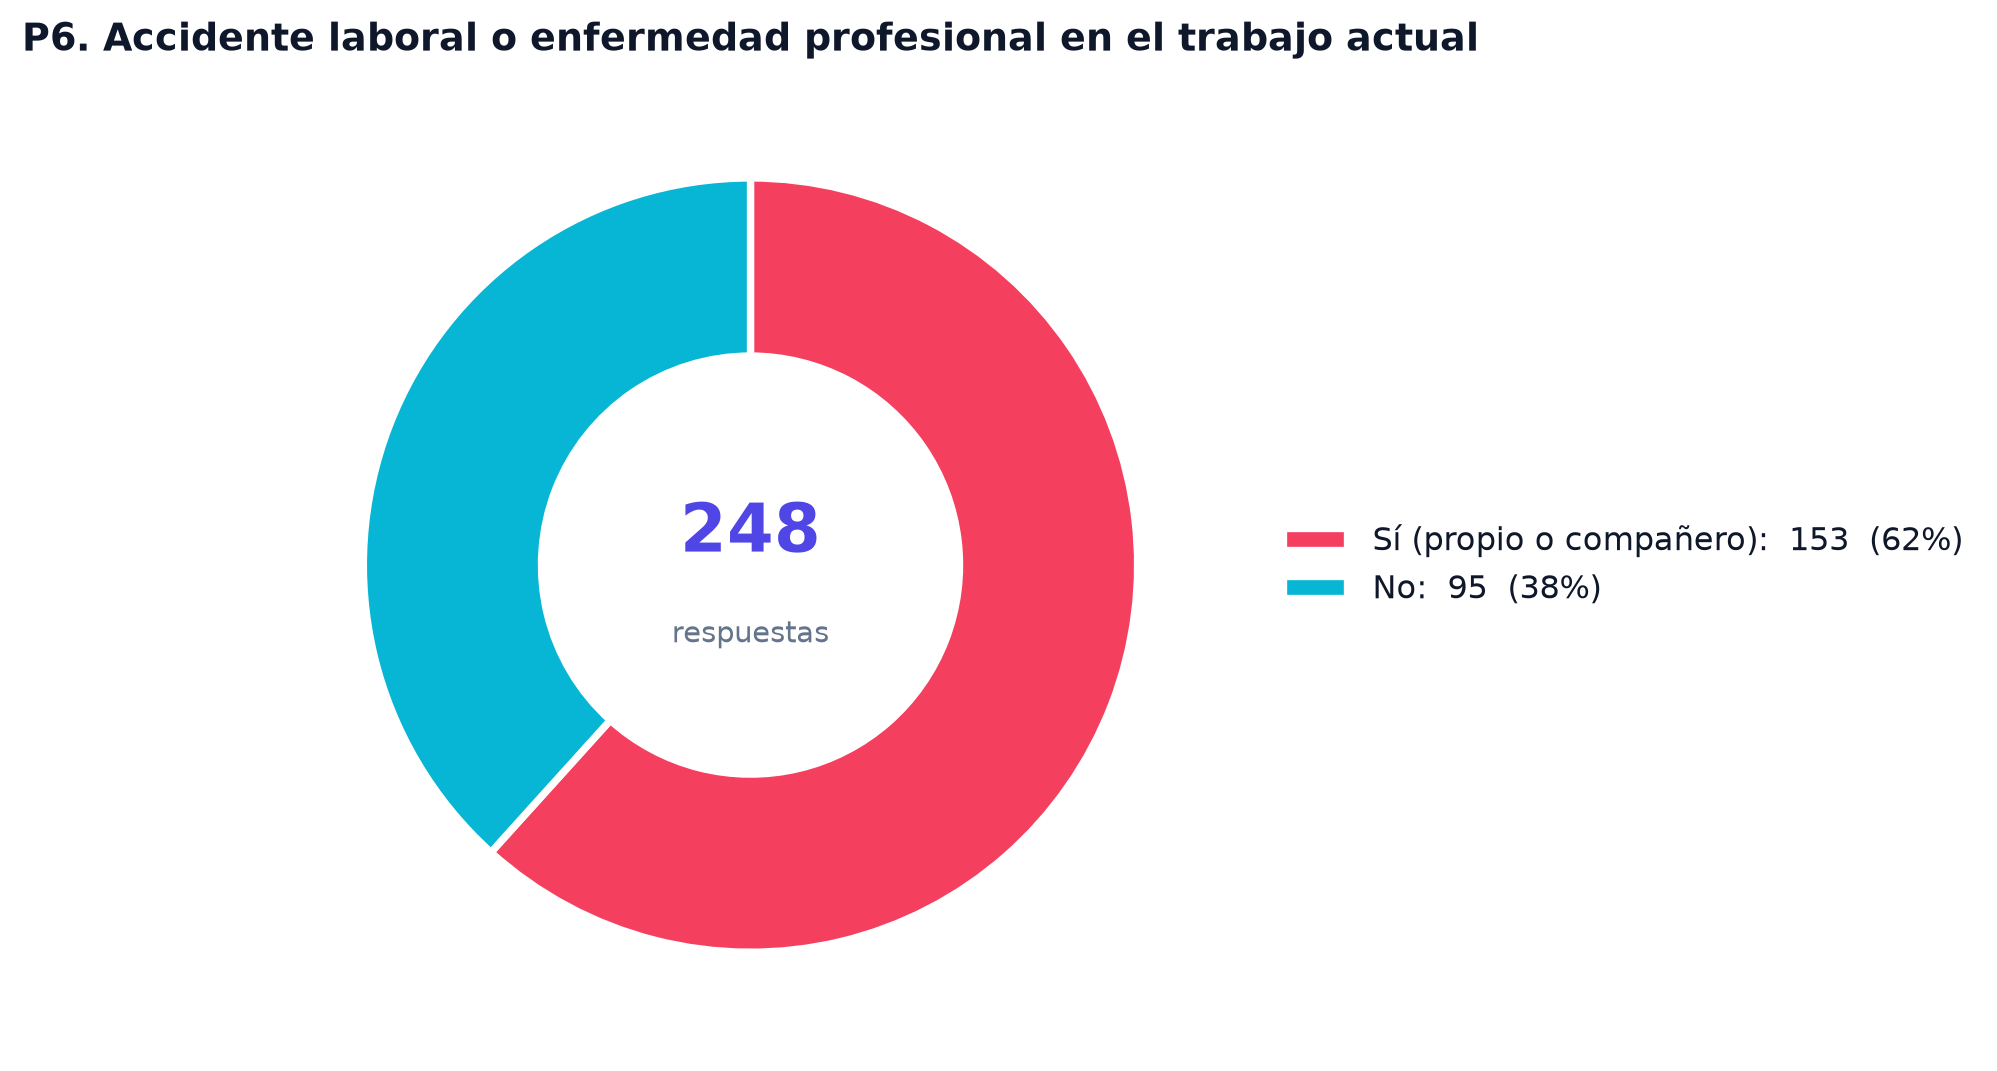
\includegraphics[width=0.88\textwidth]{figures/encuesta/p6_accidente.png}
	\caption{\enc{Experiencia de accidente laboral o enfermedad profesional, propio o de un compa\~nero. $n=248$.}}
	\label{fig:enc-p6}
\end{figure}

\enc{El 62\,\% reporta al menos un episodio en el trabajo actual.}

\subsection*{P7: Cambios operativos tras el accidente}

\begin{figure}[htbp]
	\centering
	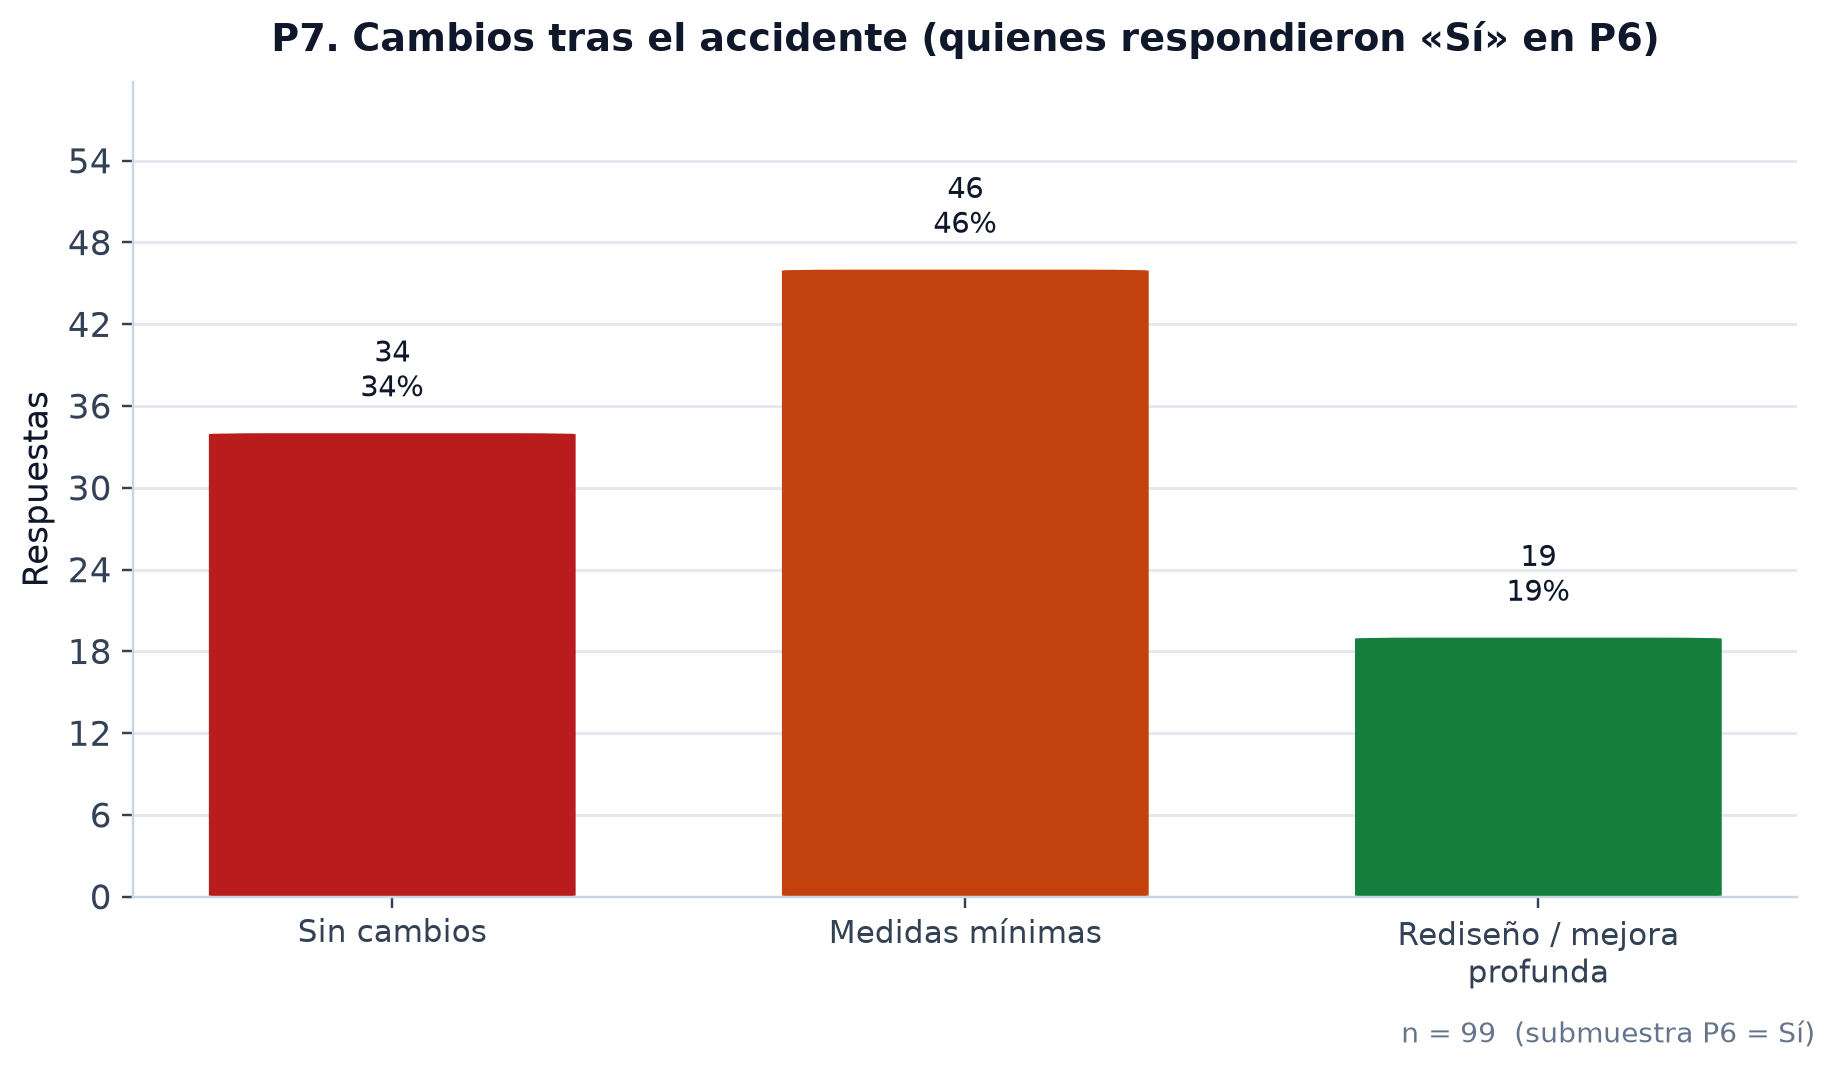
\includegraphics[width=0.92\textwidth]{figures/encuesta/p7_cambios.png}
	\caption{\enc{Cambios percibidos tras el accidente, solo quienes respondieron S\'{\i} en P6. $n=151$ v\'alidas, tras excluir No aplica residuales.}}
	\label{fig:enc-p7}
\end{figure}

\enc{El 23\,\% percibi\'o redise\~no de procesos y mejora de seguridad.
El 34\,\% indica que todo sigui\'o igual.
El 43\,\% solo medidas m\'{\i}nimas, charla o cartel.}

\subsection*{Limitaciones}

Muestra de conveniencia, sin marco muestral ART o SRT.
Autoreporte perceptivo, no auditor\'{\i}a objetiva de visitas.
Posible sesgo por las redes de difusi\'on del formulario.

\fi
\ifdeliveryannexinterviews
	\begin{contenidoNuevo}

\anexo{Transcripci\'on de entrevista --- Adri\'an El\'{\i}as}\label{anexo:entrevista-adrian-elias}

\subsection*{Ficha t\'ecnica}

\begin{description}[style=nextline, leftmargin=3.2cm, labelwidth=2.8cm]
	\item[Fecha] 6 de agosto de 2026.
	\item[Duraci\'on] Aproximadamente 20 minutos.
	\item[Modalidad] Videollamada con grabaci\'on y transcripci\'on autom\'atica posterior.
	\item[Entrevistador] Francisco Dante Mamone (autor del PFI).
	\item[Entrevistado] Adri\'an El\'{\i}as, con trayectoria operativa y funcional en una aseguradora de riesgos del trabajo (ART) y en el desarrollo del sistema \emph{core} del ramo.
	\item[Tipo] Entrevista semiestructurada (gu\'{\i}a de preguntas con posibilidad de repreguntas).
\end{description}

\noindent\textit{Nota metodol\'ogica.}
La transcripci\'on autom\'atica se depur\'o para eliminar muletillas, superposiciones y ruido de la grabaci\'on.
Las preguntas del entrevistador se reformularon en un registro formal, sin alterar el sentido de las respuestas del entrevistado.
Los t\'erminos t\'ecnicos del dominio (p\'oliza, ROAM, al\'{\i}cuota, SRT, etc.) se conservaron.

\subsection*{Transcripci\'on}

\begin{description}[style=nextline, leftmargin=0cm, labelsep=0.35cm]

\item[\textbf{Entrevistador:}]
Para comenzar, ¿podr\'{\i}a describir su trayectoria profesional en la ART o en la empresa vinculada al sistema \emph{core}, y c\'omo era una jornada t\'{\i}pica en esos roles?

\item[\textbf{Entrevistado:}]
Pas\'e por varios puestos.
Arranqu\'e como gestor de siniestros: segu\'{\i}a casos, cargaba ingresos y siniestros en el sistema y exportaba informaci\'on a la Superintendencia.
Luego gestion\'e los ex\'amenes peri\'odicos: semestralmente se volcaban listados de trabajadores expuestos a agentes de riesgo, se determinaban los estudios, se enviaban notificaciones, se daba seguimiento a su realizaci\'on y se cargaban los resultados.
Despu\'es pas\'e al \'area de contratos: altas de contratos, generaci\'on e impresi\'on de p\'olizas y env\'{\i}os; era un rol con contacto con el cliente, m\'as cercano a lo comercial.
Tambi\'en tom\'e recaudaci\'on o cobranzas: estados de cuenta, reclamos por mora, llamadas, correos y notificaciones fehacientes (incluida carta documento).
Finalmente pas\'e a sistemas: primero como soporte con perfil de analista funcional junior y, m\'as adelante, como l\'{\i}der funcional del producto ART, coordinando ---a modo de \emph{project manager}--- los desarrollos del ramo en la empresa.
En resumen, atraves\'e casi todos los estadios del circuito.

\item[\textbf{Entrevistador:}]
El foco de esta tesis est\'a en la prevenci\'on dentro de la ART.
¿Tiene experiencia o conocimiento espec\'{\i}fico en esa \'area que permita responder con fundamento?

\item[\textbf{Entrevistado:}]
S\'{\i}.
El conocimiento de prevenci\'on proviene sobre todo del tiempo en ex\'amenes peri\'odicos ---que dependen del \'area de prevenci\'on--- y del tiempo en contratos.
Los contratos est\'an muy vinculados a prevenci\'on: al formalizar el contrato hay que informar al \'area de prevenci\'on para que gestione las visitas a los establecimientos y determine los riesgos.

\item[\textbf{Entrevistador:}]
¿Qu\'e criterios se utilizaban para priorizar a qu\'e establecimiento correspond\'{\i}a una visita o una auditor\'{\i}a de prevenci\'on?
Si no lo hac\'{\i}a personalmente, ¿c\'omo se resolv\'{\i}a en la empresa?

\item[\textbf{Entrevistado:}]
En prevenci\'on el criterio central es la renovaci\'on de la p\'oliza, combinada con el riesgo asociado a la actividad de la empresa.
Las actividades se clasifican entre m\'as y menos riesgosas; la cantidad de visitas anuales obligatorias por resoluci\'on no es la misma para todas.
Adem\'as existe el relevamiento general de riesgos laborales, que puede completar el empleador y se hace una vez al a\~no al renovar el contrato, y el relevamiento de agentes de riesgo (tambi\'en anual; hay empresas no expuestas a agentes de riesgo).
El calendario de visitas se determina por la actividad: por ejemplo, una industria petrolera ---con mayor riesgo--- exige visitas m\'as frecuentes que un colegio, donde el riesgo suele asociarse a temas edilicios u otros problemas no inherentes a una actividad tan peligrosa.
Tambi\'en hay visitas gatilladas por la siniestralidad: si ocurre un siniestro que requiere investigaci\'on ---por ejemplo, un posible caso inculpable u otro tratamiento especial--- interviene el \'area de prevenci\'on en ese momento puntual.

\item[\textbf{Entrevistador:}]
¿Con qu\'e herramienta o sistema interno se gestionaba esa priorizaci\'on y la agenda de visitas?

\item[\textbf{Entrevistado:}]
Hab\'{\i}a un sistema de desarrollo interno en lenguaje Centura.
Mediante men\'us, el \'area de prevenci\'on ve\'{\i}a los contratos pr\'oximos a vencer y, con eso, sab\'{\i}a que deb\'{\i}a coordinar visitas a esos establecimientos.
Cuando hab\'{\i}a un ROAM ---un siniestro grave que requiere visita--- el sistema tambi\'en alertaba qu\'e casos deb\'{\i}an atenderse, siempre que el hecho hubiera ocurrido en un establecimiento y no en la v\'{\i}a p\'ublica o en itinerancia.
Por ese software se ve\'{\i}an tambi\'en los ex\'amenes peri\'odicos, que estaban en la \'orbita de prevenci\'on.
No hab\'{\i}a notificaciones por correo electr\'onico: la prioridad la marcaban la renovaci\'on de la p\'oliza y el criterio humano sobre esa informaci\'on.

\item[\textbf{Entrevistador:}]
¿Podr\'{\i}a aclarar el rol de la p\'oliza en este circuito? ¿Qu\'e obliga y c\'omo se relaciona con las visitas de prevenci\'on?

\item[\textbf{Entrevistado:}]
Al firmar el contrato con la ART, el empleador se obliga a cumplir las normas de seguridad e higiene adecuadas para evitar accidentes en el establecimiento, seg\'un el tipo de empresa.
Empresas de m\'as de doscientos empleados deben contar con servicio propio de seguridad e higiene; algunas m\'as chicas pero con actividades muy riesgosas tambi\'en lo requieren.
Que la visita ``dependa'' de la p\'oliza se explica porque la p\'oliza obliga tanto a la ART como al empleador a cumplir esas normas.
La visita certifica ese cumplimiento; si no se cumple, el preventor ---especialista en seguridad e higiene--- formula recomendaciones a partir de lo que detecta en el establecimiento.

\item[\textbf{Entrevistador:}]
Cuando el preventor realiza la visita y emite recomendaciones, ¿c\'omo las recibe la empresa y c\'omo se hace el seguimiento de su cumplimiento?

\item[\textbf{Entrevistado:}]
Habitualmente hay una visita y, m\'as adelante, una revisita.
El preventor genera recomendaciones ---casi siempre al menos una: por ejemplo, uso de casco en cierto sector o m\'as matafuegos en un \'area--- y elabora un informe que se entrega a la ART y al empleador.
La ART puede incrementar la al\'{\i}cuota ---lo que se le cobra al empleador--- una vez al a\~no, en la renovaci\'on, si no se cumplen las recomendaciones.
Eso tambi\'en sirve como respaldo si ocurre un accidente: se puede acreditar que se brindaron recomendaciones y que no fueron aplicadas.
Quien queda expuesta ante el regulador es la ART: si no realiza las visitas, puede recibir multa; si las realiza y igual ocurre un accidente, la ART paga el siniestro.
La SRT no suele ir contra el empleador directamente: act\'ua sobre la ART.
La ART asesora en seguridad e higiene, pero no puede obligar al empleador a ejecutar todas las recomendaciones; de ah\'{\i} la importancia de la al\'{\i}cuota y del registro documental.

\item[\textbf{Entrevistador:}]
Si la ART dispusiera de un sistema capaz de alertar mayor probabilidad de accidente en un establecimiento, ¿qu\'e datos considera \'utiles para orientar mejores recomendaciones o para priorizar la visita?

\item[\textbf{Entrevistado:}]
La ART ya tiene el historial de accidentes por establecimiento y por empresa.
Eso permite medir qu\'e es lo m\'as frecuente y anticipar recomendaciones a\'un antes de la visita.
Por ejemplo, en cosecha de frutas ---como manzaneros--- suele haber pinchazos en los ojos con las ramas: si en un establecimiento ese patr\'on se repite m\'as que en otro, ya se puede insistir en protecci\'on visual.
Son herramientas potentes: al llegar a la visita se van con recomendaciones m\'as fuertes, sin depender solo de lo que se observe en el momento.
Tambi\'en importa la frecuencia de accidentaci\'on.
Prevenci\'on no solo busca evitar accidentes: tambi\'en ayuda a prevenir fraudes; por ejemplo, patrones como ca\'{\i}das reiteradas en el \'ultimo escal\'on de una escalera, o accidentes concentrados los d\'{\i}as lunes que podr\'{\i}an corresponder a hechos del fin de semana declarados m\'as tarde.

\item[\textbf{Entrevistador:}]
¿Qu\'e obst\'aculo del proceso actual eliminar\'{\i}a o simplificar\'{\i}a para mejorar la prevenci\'on de accidentes de trabajo?

\item[\textbf{Entrevistado:}]
Un problema frecuente es que la visita la tiene que realizar un preventor de la ART.
Seg\'un la envergadura de la aseguradora, eso genera demoras: hay que visitar muchos establecimientos en un mes, coordinar con el empleador y depender de la agenda del preventor.
A nivel administrativo, ser\'{\i}a deseable ---con los recaudos legales correspondientes--- que el empleador pudiera contratar un servicio de seguridad e higiene que realice la visita, la presente y alivie a la ART de esa carga operativa.
Hay mucho componente normativo en el medio.

\item[\textbf{Entrevistador:}]
Para cerrar: sabiendo que el proyecto apunta a un sistema predictivo de priorizaci\'on de visitas, ¿hay algo adicional que considere relevante aportar?

\item[\textbf{Entrevistado:}]
En cualquier herramienta de predicci\'on de accidentes por establecimiento hay que cuidar mucho las notificaciones.
Si se predice mayor riesgo y se refuerza una acci\'on, es cr\'{\i}tico definir a qui\'en se notifica.
Avisar al empleador ciertos puntos d\'ebiles puede ``levantar la perdiz'': al enterarse de una vulnerabilidad, alguien podr\'{\i}a aprovecharla.
La confidencialidad de ese dato ---o su divulgaci\'on controlada seg\'un el caso--- es de lo m\'as importante.

\item[\textbf{Entrevistador:}]
Muchas gracias por su tiempo y por la informaci\'on.

\item[\textbf{Entrevistado:}]
De nada.

\end{description}

\end{contenidoNuevo}

\fi
